\section{Design and Implementation}
\label{sec:design}

\begin{figure*}[t]
\centering
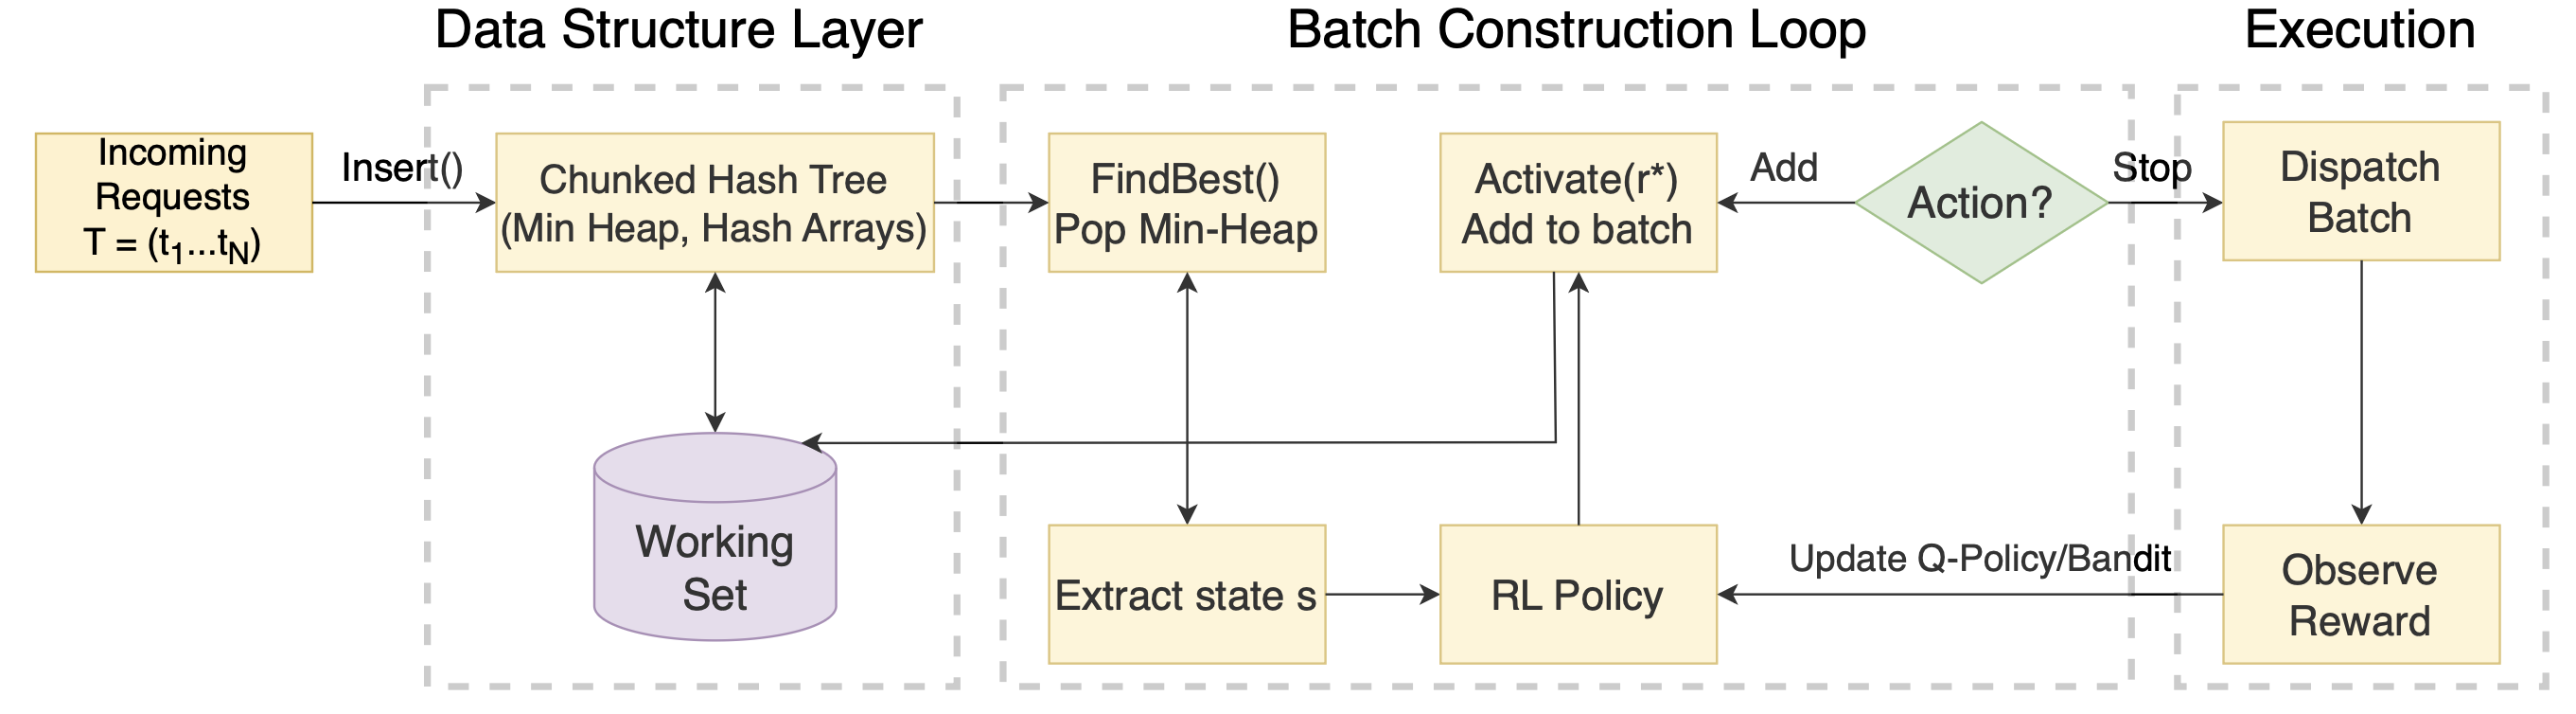
\includegraphics[width=2\columnwidth]{illustration_images/pipeline.png}
\caption{Entire Pipeline}
\label{fig:pipeline}
\end{figure*}

As shown in \S\ref{sec:motivation}, during the decode phase, memory accesses from different requests in a batch are issued almost at the same time. When all requests pass through the same KV cache in the same order, the accesses become nicely sequential, which helps the hardware prefetcher and improves effective DRAM bandwidth utilization. In this setting, as we demonstrated earlier, both temporal and spatial locality naturally emerge. However, this benefit only holds when sharing is universal across the batch. As soon as sharing becomes partial, even slightly, the reuse opportunity drops sharply. Similarly, grouping requests by prefix not only improves locality but also reduces KV cache eviction pressure, thereby preventing expensive recomputation.

\paragraph{Insight 1.} The joint objective that emerges is to keep the GPU busy while also preserving shared-prefix locality for as long as possible. A simple way to think about this is through the pair: \textbf{(Batch size, Shared prefix tokens common to all requests)}. Increasing batch size improves compute utilization. Increasing the number of shared prefix tokens across all active requests strengthens temporal and spatial locality. The goal, therefore, is not merely to build large batches, but to build large, \emph{homogeneous} batches.

\paragraph{Challenge 1.} At each step of batch formation, where we continuously add requests from the waiting queue into the running scheduler batch, there exists a trade-off between adding a new request to increase GPU utilization and maintaining temporal and spatial locality over a longer shared prefix. This trade-off is sensitive to the interplay between the GPU's compute capability and memory bandwidth, making it difficult to resolve with a fixed heuristic across different kinds of GPUs. In particular, it is unclear when to fall back from a homogeneous batch (all requests sharing a long prefix) to a heterogeneous one (mixed prefixes), especially when insufficient homogeneous requests are available in the queue. 

\paragraph{Key Idea 1.} We propose learning a reinforcement learning (RL) policy for the scheduler that adaptively resolves this trade-off at runtime, guided by the observed reward.

\paragraph{Insight 2.} Beyond scheduling, efficiently identifying which requests share a common prefix is a critical bottleneck in itself. Existing approaches to prefix detection incur significant CPU overhead, causing stalls during inference; particularly as sequence lengths grow to thousands of tokens.

\paragraph{Challenge 2.} Designing a data structure that supports fast, low-overhead prefix identification at scale is non-trivial. The structure must handle long sequences efficiently, support dynamic insertion and lookup, and impose minimal CPU cost so as not to bottleneck the inference pipeline.

\paragraph{Key Idea 2.} We introduce \emph{Chunked Hash Tree}, a data structure that detects shared prefixes with substantially lower CPU overhead than existing methods and scales well to longer sequences.



\subsection{System Overview} 
\label{sec:system_overview}
Figure~\ref{fig:pipeline} illustrates the overall pipeline of our scheduling system. The goal of the scheduler is to construct batches that both keep the GPU well utilized and preserve spatial-temporal locality for the KV cache. To achieve this, our design combines two main components:
(i) a lightweight prefix-tracking data structure called \emph{Chunked Hash Tree (CHT)} and
(ii) a learning-based policy that decides when batch construction should stop.

\paragraph{Request model.} We consider an inference server that continuously receives decoding requests. Each request consists of a prompt, which is a sequence of input tokens, followed by autoregressive decoding. At any point in time, a request falls into one of these three states: 
(i) \emph{waiting} requests that have not yet been scheduled,
(ii) \emph{active} requests that are currently part of the decoding batch, and
(iii) \emph{finished} requests whose decoding has been completed.

The scheduler operates in repeated decoding steps. During each step, it incrementally constructs a batch by selecting requests from the waiting queue and activating them. Once the batch is finalized, it is executed for one decoding iteration on the GPU.

\paragraph{Prefix-aware request selection.} The first challenge is identifying which waiting request should be added next to the batch. Ideally, we want to add requests whose prefixes overlap with those of the already active requests, since this increases temporal and spatial locality. To support this efficiently, we introduce \emph{Chunked Hash Tree}. Instead of comparing token sequences directly, each request is represented using a compact vector of cumulative prefix hashes computed at fixed token intervals. These hashes allow the scheduler to quickly detect shared prefixes across requests. The CHT maintains a working set that represents the prefixes currently referenced by active requests and tracks how much prefix overlap each waiting request has with this working set. Using this information, the scheduler can efficiently identify the waiting request that maximizes our joint objective function.

\paragraph{Batch construction loop.} Using the CHT, the scheduler repeatedly retrieves the best candidate request from the waiting queue (the one with the highest prefix overlap) and considers adding it to the current batch. Each candidate provides useful statistics, such as the current batch size, the shared-prefix length across all active requests before and after the addition, and the number of waiting requests that could benefit from the same prefix. At this point, the scheduler must decide whether to add the request or stop building the batch. Adding more requests improves GPU utilization but may reduce prefix locality if the shared prefix becomes smaller.

\paragraph{Learning when to stop.} We formulate this decision as a learning problem. The scheduler observes a state that summarizes the current batch size and prefix-sharing statistics, and a reinforcement learning policy chooses between two actions: \textsc{Add} the candidate request to the batch or \textsc{Stop} and dispatch the batch for execution. After the batch is executed, the system observes the resulting performance (e.g., throughput) and uses it as feedback to update the policy. Over time, the policy learns how to balance GPU utilization and prefix locality for different workload conditions.

\paragraph{End-to-end flow.} Putting everything together, the pipeline works as follows. Incoming requests are first inserted into the CHT, where their prefix hashes are computed and indexed. During batch construction, the scheduler repeatedly calls \textsc{FindBest} to retrieve the best candidate request based on prefix overlap. The reinforcement learning policy then decides whether to activate the request and add it to the batch or to stop. Once the batch is finalized, it is dispatched for execution on the GPU. The observed throughput is then used to update the policy for future scheduling decisions. 

The following subsections describe the Chunked Hash Tree data structure in detail and then present the batching and reinforcement learning policies built on top of it.

\subsection{Chunked Hash Tree}
\textcolor{red}{a better name, without a tree, for uniqueness. Do we need to make it a separate section?}

\textcolor{red}{starting with a brief overview}

\textcolor{red}{need to mention that implemented in C++ (can do so in the section integration with vllm)}

\begin{figure*}[t]
\centering
\begin{subfigure}{0.32\textwidth}
    \centering
    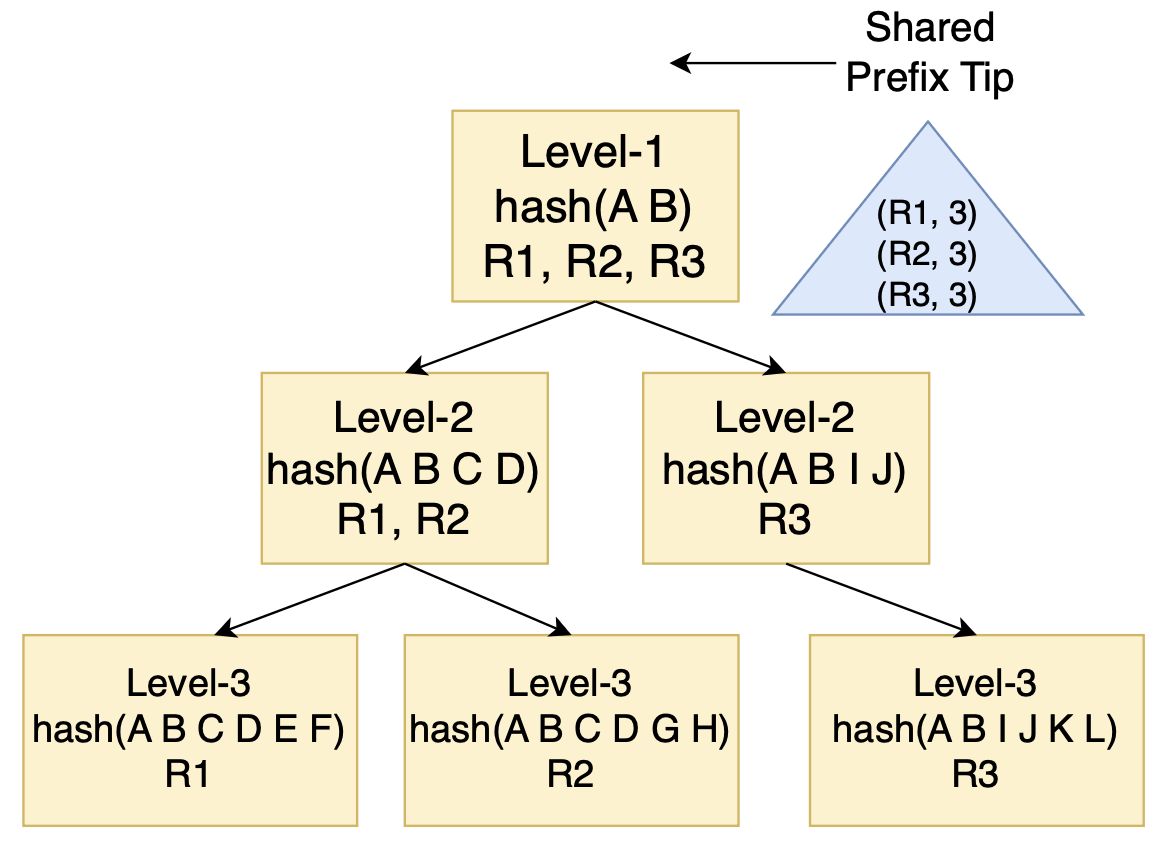
\includegraphics[width=\linewidth]{illustration_images/chunked_hash_tree_insertion.png}
    \caption{}
    \label{fig:chunked_hash_tree_insertion}
\end{subfigure}
\hfill
\begin{subfigure}{0.32\textwidth}
    \centering
    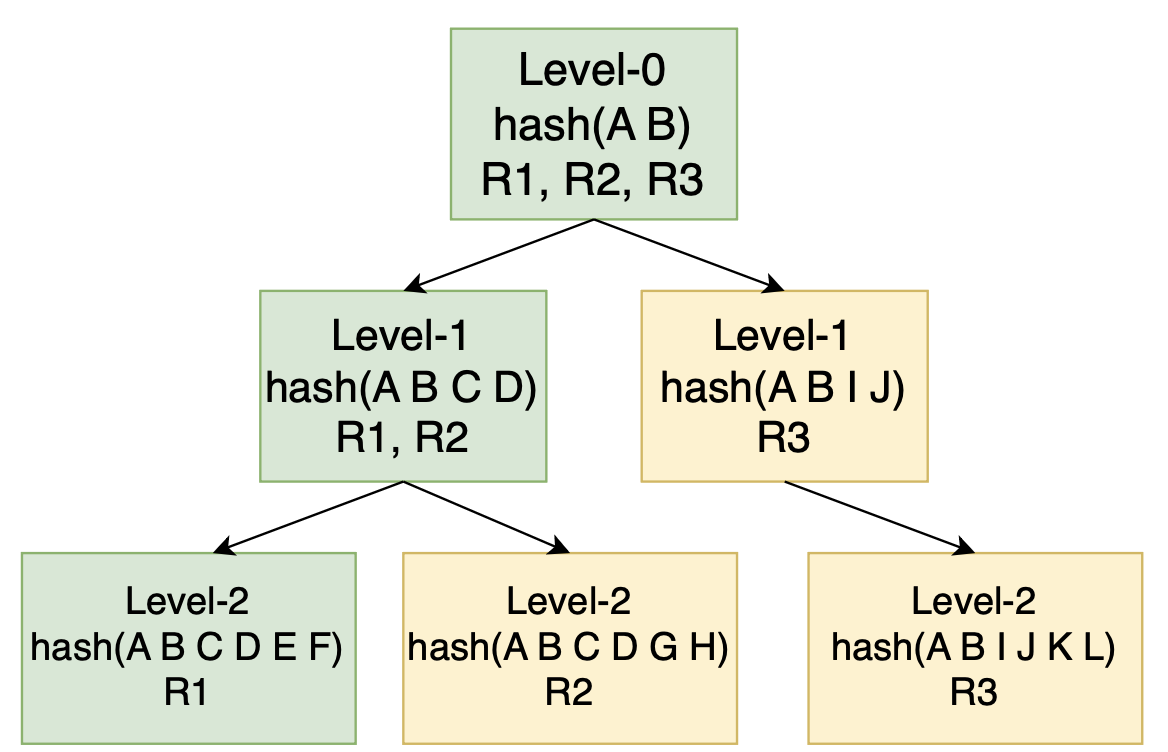
\includegraphics[width=\linewidth]{illustration_images/chunked_hash_tree_activation.png}
    \caption{}
    \label{fig:chunked_hash_tree_activation}
\end{subfigure}
\hfill
\begin{subfigure}{0.32\textwidth}
    \centering
    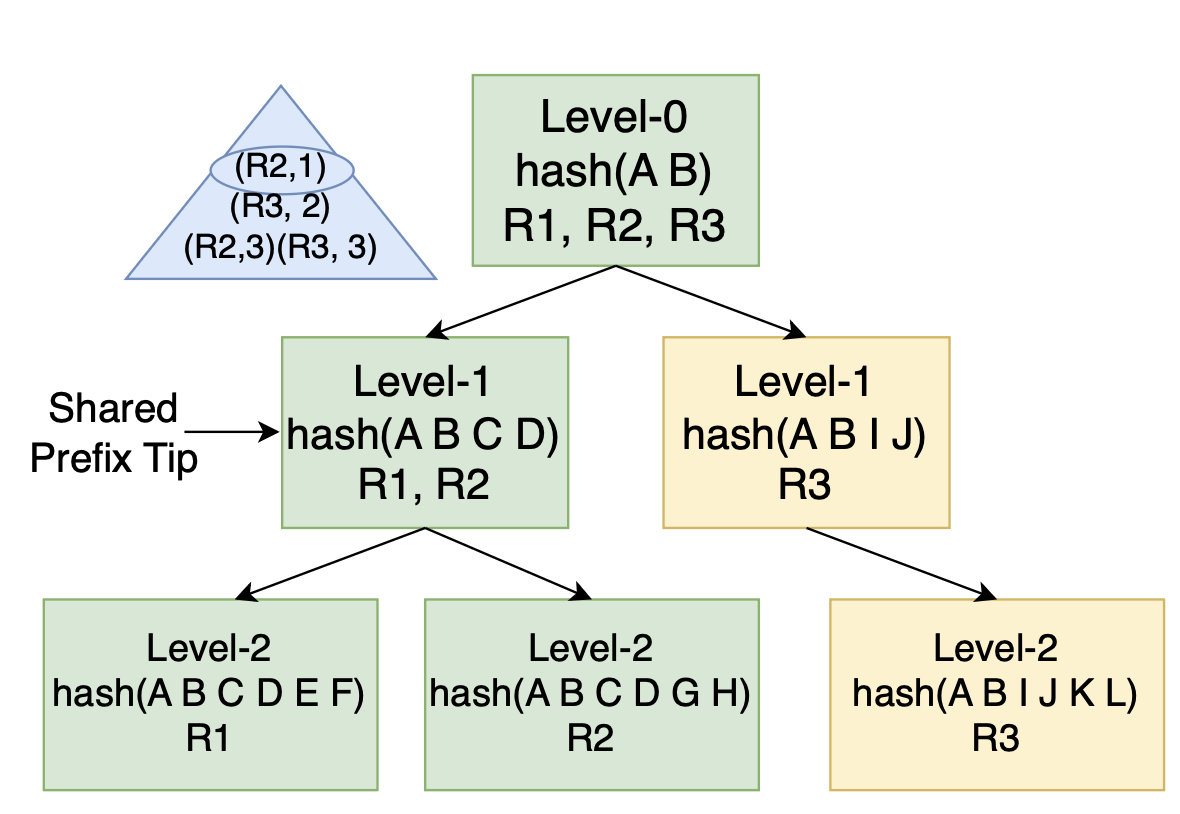
\includegraphics[width=\linewidth]{illustration_images/chunked_hash_tree_find_best_request.png}
    \caption{}
    \label{fig:chunked_hash_tree_find_best_request}
\end{subfigure}

\caption{An example of chunked hash tree workflow which shows insertion, activation and best request selection. Consider 3 requests $R_1, R_2, R_3$ each with 6 tokens. With a chunk size of 2, each request will get divided into 3 levels, as shown in~\ref{fig:chunked_hash_tree_insertion}. Next, we add $R_1$ to the active decoding batch, this makes the shared prefix chain include all its nodes, which are marked as green in ~\ref{fig:chunked_hash_tree_activation}. Now, we wish to find the next candidate request which can be added to the running batch. We have two options $R_2$ and $R_3$. Since, $R_2$ has the max overlap with the current shared prefix chain, we prefer it over $R_3$, as shown in~\ref{fig:chunked_hash_tree_find_best_request}.}
\label{fig:chunked_hash_tree_workflow}
\end{figure*}


\subsubsection*{Motivation and Design Evolution} The scheduler repeatedly needs to answer a simple question: among all waiting requests, which one shares the largest prefix with the currently active batch? Requests that share longer prefixes will lead to higher temporal and spatial locality. Since scheduling decisions occur frequently and the waiting queue may contain thousands of requests with long prompts, detecting prefix overlap must be extremely fast and impose minimal CPU overhead.

Modern inference systems already exploit prefix sharing for KV-cache reuse. As shown in \S\ref{sec:background}, vLLM~\cite{kwon2023efficient} uses Merkle Trees, while SGLang~\cite{zheng2024sglangefficientexecutionstructured} and BatchLLM~\cite{zheng2025batchllmoptimizinglargebatched} use radix trees to detect prefix sharing. Our scheduler, however, has a different objective: we do not need to store or manage KV-cache blocks; instead, we only need a lightweight way to estimate how much prefix overlap exists between requests so that we can select the best request to add to the batch. While a radix tree precisely captures prefix sharing, it incurs significant overhead; every insertion may trigger node splitting, and finding the best matching waiting request requires a DFS traversal that is $O(W)$ in the worst case, where $W$ is the number of waiting requests. For a scheduler making frequent decisions over thousands of long-prompt requests, that is quite expensive. Similarly, Merkle-style hash chains introduce unnecessary sequential dependencies during hash computation and expose more structure than the scheduler actually requires.

We instead want a structure centered around a \emph{working set}: the set of prefix chunks currently held by active requests; so that we can directly ask: ``which waiting request has the most overlap with the already running batch?'' This reframes the problem from tree traversal to set intersection. To that end, rather than maintaining a strict hash chain, we divide the token sequence into fixed-size chunks and compute prefix hashes at chunk boundaries. An additional advantage of this design is that hash computation can be naturally batched and parallelized. Because chunks are processed independently, their hash contributions can be computed separately and later combined to obtain the cumulative prefix hashes. This pattern is similar in spirit to techniques such as online softmax, where partial statistics are computed over blocks and then merged to produce the final result. In contrast, Merkle-style hash chains require sequential computation because each hash depends on the previous one.

The simplest realization is to represent each request as a set of hashed prefix chunks, maintain the working set explicitly, and, on each scheduling decision, scan all waiting requests and count how many of their chunks appear in the working set. The request with the highest overlap wins. This is correct and easy to implement, but finding the best request is $O(W \cdot C)$ --- linear in the number of waiting requests times chunks per request, since we rescan everything on every call.

We can avoid rescanning by maintaining a \emph{missing count} per waiting request: the number of its chunks that are absent from the working set. This count only needs to change when the working set itself changes, i.e., upon activation or completion of a request. Instead of recomputing overlaps from scratch, we propagate small delta updates. Finding the best request then becomes a linear scan over waiting requests to find the minimum missing count — $O(W)$.

To eliminate the linear scan, we maintain a min-heap ordered by missing count. When a chunk enters or leaves the working set, we update the missing counts of affected waiting requests and push new entries to the heap. However, in-place heap updates are expensive, so we use \emph{lazy deletion}: push a new entry with the updated count, and skip stale entries (where the heap's recorded count differs from the current missing cache) when popping. This reduces the complexity to $O(\log W)$ amortized, while keeping activation and completion costs proportional only to the number of \emph{affected} waiting requests per chunk—typically far smaller than $W$.

The resulting structure, which we call the \emph{Chunked Hash Tree} (CHT), is a scheduling data structure that maximizes KV-cache prefix reuse across concurrent inference requests. We first describe how requests are represented as hash vectors, then introduce the data structures that track the scheduler state, and finally walk through each operation in turn.


\subsubsection*{Hash Computation}
Before a request can be inserted into the scheduler, its token sequence must be converted into a compact representation that captures the prefix-sharing structure.  As shown in Figure~\ref{fig:chunked_hash_tree_prefix_representation}, given a request with a token sequence $T = (t_1, t_2, \dots, t_N)$, we partition $T$ into non-overlapping chunks of size $K$ (e.g., $K = 50$). For each chunk boundary $\ell = 1, \dots C$ where $C = \lceil N/K \rceil$, we compute a \emph{cumulative prefix hash} at each boundary\\ $h_\ell = \mathrm{hash}(t_1, t_2, \dots, t_{\min(\ell K,\, N}), \quad \ell = 1, \dots, C$.

Because the hash is cumulative, two requests share the same $h_\ell$ if and only if their first $\ell K$ tokens are identical, which is precisely the condition under which their KV-cache prefixes can be shared. Each request $r$ is therefore represented as an ordered hash vector $H_r = (h_1^r, h_2^r, \dots, h_C^r)$.

Algorithm~\ref{alg:compute_hashes} details the hash computation. We use an incremental xxHash-64 state so that each token is processed exactly once, making the total cost $O(N)$ regardless of the number of chunked boundaries.

\begin{algorithm}[H]
\caption{$\textsc{ComputeHashes}(T, K)$}
\label{alg:compute_hashes}
\begin{algorithmic}[1]
\Require Token sequence $T = (t_1, \dots, t_N)$; chunk size $K$
\Ensure Cumulative prefix-hash vector $H = (h_1, \dots, h_C)$
\State $H \gets []$;\quad $C \gets \lceil N / K \rceil$
\State Initialise incremental \textsc{xxHash-64} state $s$
\For{$i \gets 1$ \textbf{to} $N$}
  \State Feed $t_i$ into $s$
  \If{$i \bmod K = 0$ \textbf{or} $i = N$}
    \State $H.\textsc{Append}(\textsc{Digest}(s))$
  \EndIf
\EndFor
\State \Return $H$
\end{algorithmic}
\end{algorithm}

\begin{figure}[H]
\centering
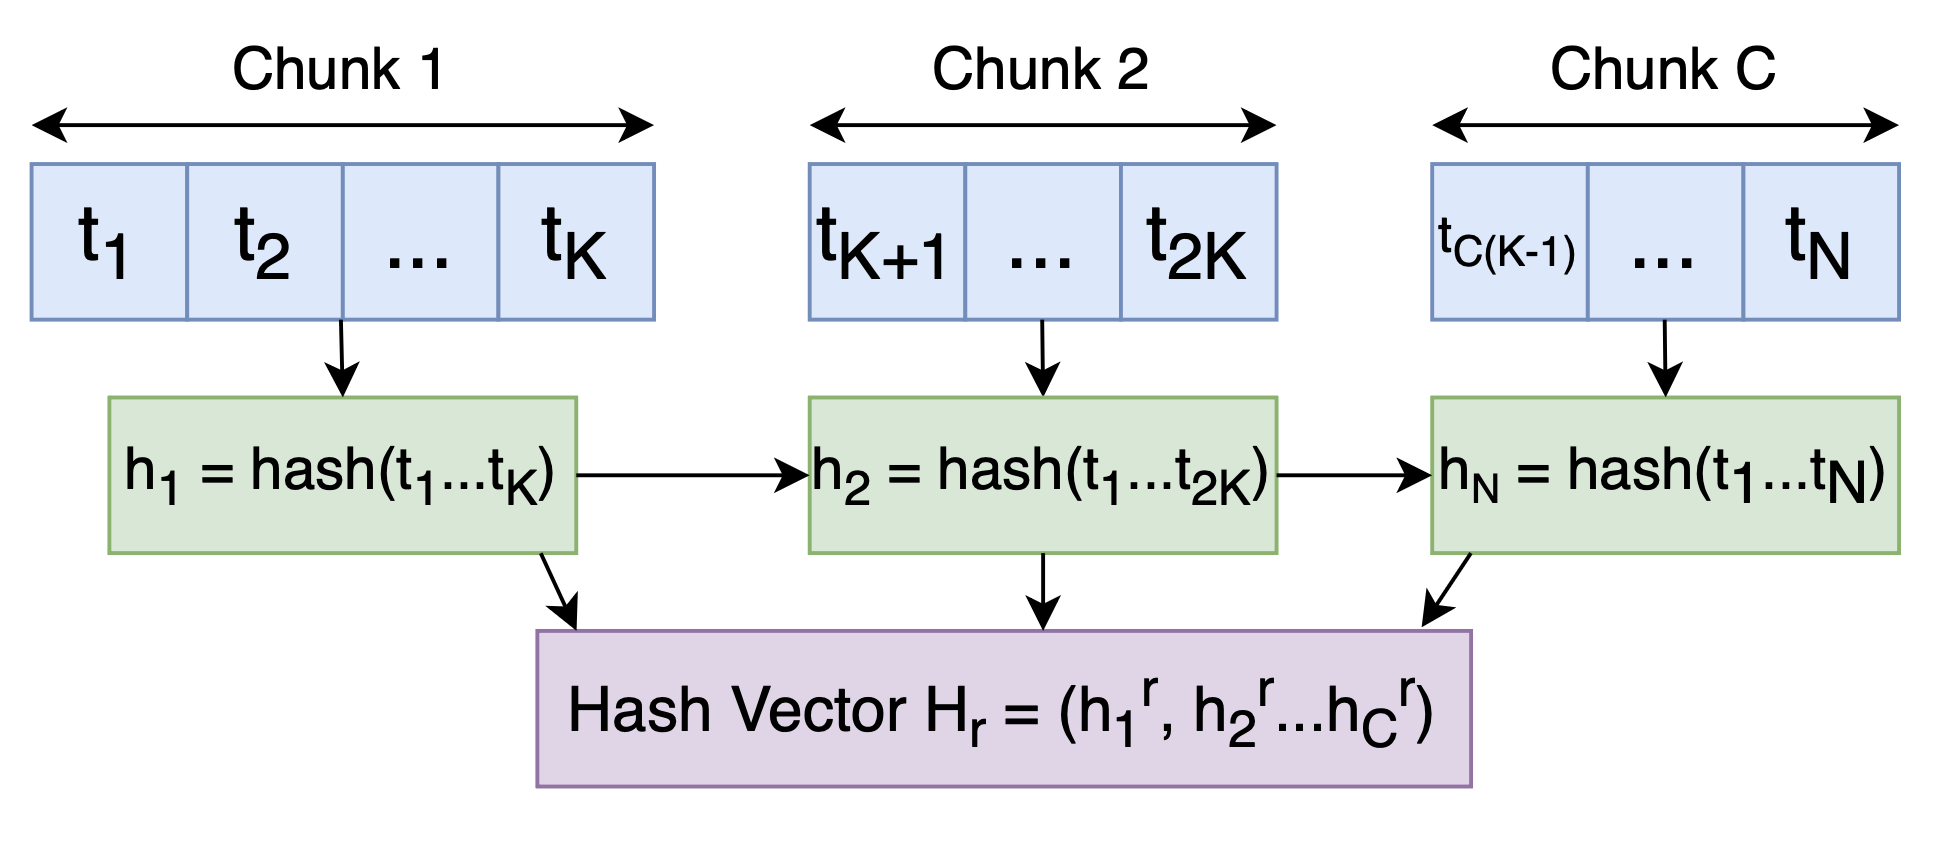
\includegraphics[width=\columnwidth]{illustration_images/chunked_hash_tree_prefix_representation.png}
\caption{Hash Computation in Chunked Hash Tree}
\label{fig:chunked_hash_tree_prefix_representation}
\end{figure}

\subsubsection*{Data Structures}
The CHT maintains the following components that together capture the full scheduler state:

\paragraph{Hash vectors.} A map from request ID to its cumulative prefix-hash vector $H_r = (h_1^r, \dots, h_C^r)$ is stored for every active and waiting request.

\paragraph{Reference counts.} \texttt{ref} maps each $h$ to the number of currently \emph{active} requests that contain that hash in their hash vectors. 

\paragraph{Working set.} \texttt{working\_set} is the set of hashes that belong to at least one \emph{active} request. A hash is in the working set if and only if its reference count is greater than zero.

\paragraph{Missing cache.} \texttt{miss} maps each \emph{waiting} request $r$ to an integer $m_r$, defined as the number of hashes in $H_r$ that are \emph{not} currently in the working set. Intuitively, $m_r$ counts how many of $r$'s prefix chunks would need to be freshly computed (i.e., are not already cached by the active batch). A request with $m_r = 0$ has its entire prefix covered by the current active batch and is therefore the most preferable candidate to admit next.

\paragraph{Waiting heap.} \texttt{waiting\_heap} is a min-heap of $(m_r, r)$ pairs, ordered by missing count $m_r$. It enables $O(\log W)$ retrieval of the waiting request with the smallest missing count, where $W$ is the number of waiting requests.

\paragraph{Reverse index.} \texttt{waiting} maps each hash $h$ to the set of waiting requests whose hash vector contains $h$, enabling $O(1)$ updates to \texttt{miss} when the working set changes.

\paragraph{Shared prefix chain.} \texttt{shared\_prefix\_chain} is a vector $P = (p_1, \dots, p_L)$ recording the longest common hash prefix shared by all currently active requests. $P$ is maintained incrementally rather than recomputed from scratch for every event, keeping the amortized cost low. 


\subsubsection*{Request Insertion (Algorithm~\ref{alg:insert})}
$\textsc{Insert}$ is called the moment a new request arrives at the scheduler. It computes $H_r$ via $\textsc{ComputeHashes}$, stores the hash vector, and for each hash $h \in H_r$, registers $r$ in the reverse index $\mathit{waiting}[h]$. Crucially, it also computes the initial missing count $m_r$: the number of hashes in $H_r$ not yet present in the working set. This count is stored in $\mathit{miss}[r]$ and the pair $(m_r, r)$ is pushed onto the waiting heap. No reference counts are modified at this stage; that happens only when the request is activated.

\begin{algorithm}[H]
\caption{$\textsc{Insert}(r, T)$}
\label{alg:insert}
\begin{algorithmic}[1]
\Require Request $r$; token sequence $T$; working set $\mathit{working\_set}$; reverse index $\mathit{waiting}$; min-heap $\mathit{waiting\_heap}$
\Ensure $r$ registered and ready for scheduling
\State $H_r \gets \textsc{ComputeHashes}(T, K)$
\State $\mathit{request\_hashes}[r] \gets H_r$
\State $m_r \gets 0$
\State $\mathit{waiting\_requests} \gets \mathit{waiting\_requests} \cup \{r\}$
\For{$\ell \gets 1$ \textbf{to} $|H_r|$}
  \If{$h_\ell^r \notin \mathit{working\_set}$}
    \State $m_r \gets m_r + 1$
  \EndIf
  \State $\mathit{waiting}[h_\ell^r] \gets \mathit{waiting}[h_\ell^r] \cup \{r\}$
\EndFor
\State $\mathit{miss}[r] \gets m_r$
\State $\mathit{waiting\_heap}.\textsc{Push}(m_r,\; r)$
\end{algorithmic}
\end{algorithm}

\paragraph{Activation (Algorithm~\ref{alg:activate}).} 
$\textsc{Activate}$ is called when the scheduler moves a request from the waiting queue into the active decoding batch. For each hash $h$ in $H_r$, if $h$ transitions from absent to present in the working set (i.e., its reference count goes from 0 to 1), then $h$ is added to the working set and all waiting requests that contain $h$ have their missing count decremented by one; updated pairs are pushed onto the heap. This eager propagation keeps $\mathit{miss}$ accurate for all waiting requests without requiring a full rescan. The shared prefix chain is then updated incrementally via $\textsc{UpdateChainOnActivate}$ (Algorithm~\ref{alg:update_chain_activate}).

\begin{algorithm}[H]
\caption{$\textsc{Activate}(r)$}
\label{alg:activate}
\begin{algorithmic}[1]
\Require Request $r$ with hash vector $H_r$; ref counts $\mathrm{ref}$; working set $\mathit{working\_set}$; reverse index $\mathit{waiting}$; missing cache $\mathit{miss}$; min-heap $\mathit{waiting\_heap}$
\Ensure Updated $\mathrm{ref}$, $\mathit{working\_set}$, $\mathit{miss}$; updated shared prefix chain
\State $\mathit{waiting\_requests} \gets \mathit{waiting\_requests} \setminus \{r\}$;
\State       $\mathit{active} \gets \mathit{active} \cup \{r\}$
\State $\mathit{added} \gets 0$
\For{$\ell \gets 1$ \textbf{to} $|H_r|$}
  \If{$\mathrm{ref}[h_\ell^r] = 0$}
  \Comment{$h_\ell^r$ newly enters working set}
  \State $\mathit{working\_set} \gets \mathit{working\_set} \cup \{h_\ell^r\}$
  \For{$w \in \mathit{waiting}[h_\ell^r]$}
      \If{$w \notin \mathit{active}$ \textbf{and} $w \in \mathit{miss}$}
        \State $\mathit{miss}[w] \gets \mathit{miss}[w] - 1$
        \State $\mathit{waiting\_heap}.\textsc{Push}(\mathit{miss}[w],\; w)$
      \EndIf
    \EndFor
    \State $\mathit{added} \gets \mathit{added} + 1$
  \EndIf
  \State $\mathrm{ref}[h_\ell^r] \gets \mathrm{ref}[h_\ell^r] + 1$
\EndFor
\State $\textsc{UpdateChainOnActivate}(r)$
\State \Return $(\mathit{added},\; |H_r|)$
\end{algorithmic}
\end{algorithm}

\paragraph{Updating the shared prefix chain on activation (Algorithm~\ref{alg:update_chain_activate}).}
It is called at the end of every $\textsc{Activate}$ after $r$ has been added to the active set. It keeps the shared prefix chain consistent without recomputing it from scratch. Because adding a new request can only \emph{shorten} the common prefix (never lengthen it), we must find the longest prefix of the current chain $P$ that $H_r$ also satisfies.

As described before, each hash $h_\ell$ is produced by a cumulative (prefix) hasher: $h_\ell$ is the digest of all tokens from position $1$ through $\ell \cdot C$, where $C$ is the chunk size. Consequently, if two hash vectors agree at level $\ell$, they necessarily agree at every level $1, \ldots, \ell-1$ as well, because those earlier digests are sub-sequences of the same cumulative stream. Formally, we define the predicate $\mathcal{M}(\ell) \;=\; \bigl[h_\ell^r = p_\ell\bigr]$. The cumulative property guarantees that $\mathcal{M}$ is \emph{monotone decreasing} on the index set $\{1, \dots, \min(L, |H_r|)\}$: once $\mathcal{M}(\ell)$ is false for some $\ell^*$, it is false for all $\ell > \ell^*$. This monotone structure is exactly the condition required for binary search to be correct: we seek the largest $k$ such that $\mathcal{M}(k)$ is true, and binary search finds it in $O(\log \min(L, |H_r|))$ comparisons rather than the $O(\min(L, |H_r|))$ required by a linear scan.

\begin{algorithm}[H]
\caption{$\textsc{UpdateChainOnActivate}(r)$}
\label{alg:update_chain_activate}
\begin{algorithmic}[1]
\Require Request $r$ with hash vector $H_r$; current shared chain $P$ of length $L$; active set $\mathit{active}$
\Ensure $P$ reflects the longest common prefix of all active requests
\If{$|\mathit{active}| = 1$}
    \Comment{$r$ is the only active request}
    \State $P \gets H_r$;\quad $L \gets |H_r|$
    \State \Return
\EndIf
\State $L \gets \textsc{BinarySearch}\!\left(H_r,\, P,\, \min(L,\, |H_r|)\right)$
\Comment{largest $k$ s.t.\ $h_k^r = p_k$}
\State Truncate $P$ to its first $L$ entries
\end{algorithmic}
\end{algorithm}

\paragraph{Completion (Algorithm~\ref{alg:finish}).} $\textsc{Finish}$ is called when the model has generated the final token for request $r$, and the request is removed from the active batch. For each hash $h$ in $H_r$, its reference count is decremented; if it reaches zero, $h$ is evicted from the working set, and all waiting requests containing $h$ have their missing count incremented by one, with updated pairs pushed onto the heap. The shared prefix chain is then updated via $\textsc{UpdateChainOnFinish}$, since removing a request can only lengthen the common prefix.


\begin{algorithm}[H]
\caption{$\textsc{Finish}(r)$}
\label{alg:finish}
\begin{algorithmic}[1]
\Require Request $r$ with hash vector $H_r$; ref counts $\mathrm{ref}$; working set $\mathit{working\_set}$; reverse index $\mathit{waiting}$; missing cache $\mathit{miss}$; min-heap $\mathit{waiting\_heap}$
\Ensure Updated $\mathrm{ref}$, $\mathit{working\_set}$, $\mathit{miss}$; reverse index cleaned; updated shared prefix chain
\State $\mathit{active} \gets \mathit{active} \setminus \{r\}$
\State $\mathit{evicted} \gets 0$
\For{$\ell \gets 1$ \textbf{to} $|H_r|$}
  \State $\mathrm{ref}[h_\ell^r] \gets \mathrm{ref}[h_\ell^r] - 1$
   \If{$\mathrm{ref}[h_\ell^r] = 0$}
   \State $\mathit{working\_set} \gets \mathit{working\_set} \setminus \{h_\ell^r\}$
    \For{$w \in \mathit{waiting}[h_\ell^r]$}
      \If{$w \notin \mathit{active}$ \textbf{and} $w \in \mathit{miss}$}
        \State $\mathit{miss}[w] \gets \mathit{miss}[w] + 1$
        \State $\mathit{waiting\_heap}.\textsc{Push}(\mathit{miss}[w],\; w)$
      \EndIf
    \EndFor
    \State $\mathit{evicted} \gets \mathit{evicted} + 1$
  \EndIf
\EndFor
\State $\textsc{UpdateChainOnFinish}(r)$
\State $\textsc{Remove}(r)$
  \Comment{cleans $\mathit{waiting}$ index and $\mathit{request\_hashes}$}
\State \Return $(\mathit{evicted},\; |H_r|)$
\end{algorithmic}
\end{algorithm}

\paragraph{Updating the shared prefix chain on completion (Algorithm~\ref{alg:update_chain_finish})}
It is called inside $\textsc{Finish}$, \emph{before} $r$'s hash vector is erased, after $r$ has been removed from the active set. Removing a request can only \emph{extend} the common prefix. We therefore try to grow the chain level by level beyond its current length by checking whether all remaining active requests agree on each successive hash. Two special cases are handled up front: if no requests remain, the chain is cleared; if exactly one request remains, the chain is set to its full hash vector.

\begin{algorithm}[H]
\caption{$\textsc{UpdateChainOnFinish}(r)$}
\label{alg:update_chain_finish}
\begin{algorithmic}[1]
\Require Active set $\mathit{active}$ (already excludes $r$); current shared chain $P$ of length $L$; hash vectors $\mathit{request\_hashes}$
\Ensure $P$ extended as far as all remaining active requests agree
\If{$\mathit{active} = \emptyset$}
\State $P \gets []$;\quad $L \gets 0$;\quad \Return
\EndIf
\If{$|\mathit{active}| = 1$}
  \State $\textsc{RecomputeChain}()$;\quad \Return
  \Comment{sets $P$ to the sole remaining request's full hash vector}
\EndIf
\State $M \gets \min_{q \in \mathit{active}} |H_q|$
  \Comment{maximum possible extension}
\For{$\ell \gets L + 1$ \textbf{to} $M$}
  \State $h^* \gets h_\ell^{q_0}$ for an arbitrary $q_0 \in \mathit{active}$
  \If{$\forall\, q \in \mathit{active} : h_\ell^q = h^*$}
    \State $P.\textsc{Append}(h^*)$;\quad $L \gets L + 1$
  \Else
    \State \textbf{break}
  \EndIf
\EndFor
\end{algorithmic}
\end{algorithm}
 




\subsubsection*{Finding the Best Request (Algorithm~\ref{alg:find_best})}
$\textsc{FindBest}$ is called by the batch-construction loop whenever the scheduler needs to select the next candidate request to admit. The key insight is that the best candidate is the waiting request whose prefix chunks are \emph{most covered} by the current active batch, i.e., the one with the smallest missing count $m_r$. The algorithm extracts the minimum-missing-count entry from the waiting heap, skipping stale entries (those whose recorded missing count no longer matches $\mathit{miss}$ due to lazy deletion). Three auxiliary statistics are then computed to guide the caller's admission decision: 
(i) $\mathit{chunks\_before}$, the shared prefix chain length before the candidate is admitted; 
(ii) $\mathit{chunks\_after}$, the chain length that would result after admitting the candidate, computed by comparing $H_{r^*}$ with $P$; and 
(iii) $\mathit{peers}$, the number of other waiting requests sharing the prefix up to level $\mathit{chunks\_after}$, indicating the future benefit that the admission would unlock.

The result is cached and reused on repeated calls until the working set or waiting queue changes, avoiding redundant heap traversals.

\begin{algorithm}[H]
\caption{$\textsc{FindBest}()$}
\label{alg:find_best}
\begin{algorithmic}[1]
\Require Min-heap $\mathit{waiting\_heap}$ of $(m_r, r)$ pairs; missing cache $\mathit{miss}$; active set $\mathit{active}$; shared chain $P$ of length $L$
\Ensure $(r^*,\;\mathit{chunks\_before},\;\mathit{chunks\_after},\;\mathit{peers})$ or $\bot$ if the waiting queue is empty
\If{$\mathit{waiting\_requests} = \emptyset$}\ \Return $\bot$
\EndIf
\If{$\mathit{cache\_valid}$}\ \Return $\mathit{cached\_result}$
\EndIf
\While{$\mathit{waiting\_heap} \neq \emptyset$}
\State $(m, r) \gets \mathit{waiting\_heap}.\textsc{Pop}()$
  \If{$r \in \mathit{active}$}\ \textbf{continue}
    \Comment{already activated}
  \EndIf
  \If{$r \notin \mathit{miss}$}\ \textbf{continue} \Comment{request no longer exists}
  \EndIf
  \If{$\mathit{miss}[r] \neq m$}\ \textbf{continue}
    \Comment{stale heap entry}
  \EndIf
  \State $r^* \gets r$
  \State $\mathit{chunks\_before} \gets L$
  \State $\mathit{chunks\_after} \gets \textsc{ChainLengthWith}(r^*)$
    \Comment{compare $H_{r^*}$ with $P$}
  \State $\mathit{peers} \gets \textsc{WaitersAtLevel}(\mathit{chunks\_after})$
  \State $\mathit{waiting\_heap}.\textsc{Push}(m, r^*)$
    \Comment{restore entry for future calls}
  \State Cache and \Return $(r^*,\;\mathit{chunks\_before},\;\mathit{chunks\_after},\;\mathit{peers})$
\EndWhile
\State \Return $\bot$
\end{algorithmic}
\end{algorithm}


Figure~\ref{fig:chunked_hash_tree_workflow} shows a worked example of insertion,
activation, and best-request selection. Figure~\ref{fig:shared_prefix_chain_workflow} shows how the shared prefix chain shrinks and extends upon activation and completion of requests.


\begin{figure*}[t]
\centering
\begin{subfigure}{0.24\textwidth}
    \centering
    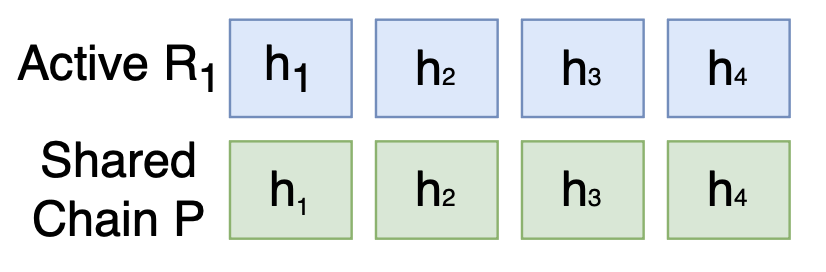
\includegraphics[width=\linewidth]{illustration_images/shared_prefix_chain_step1.png}
    \caption{}
    \label{fig:shared_prefix_chain_step1}
\end{subfigure}
\hfill
\begin{subfigure}{0.24\textwidth}
    \centering
    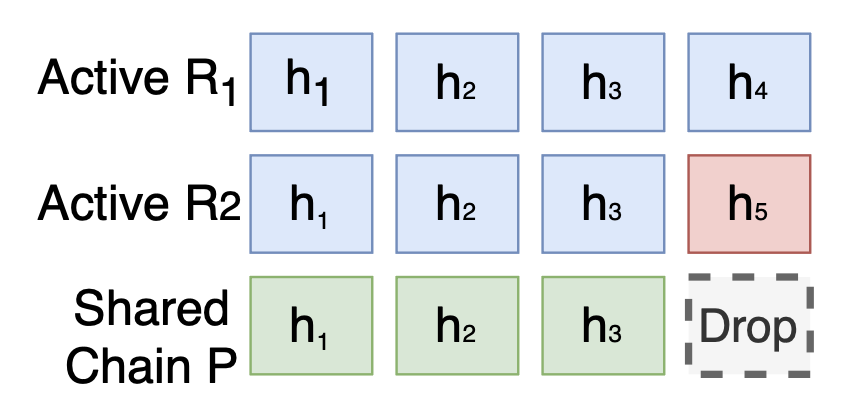
\includegraphics[width=\linewidth]{illustration_images/shared_prefix_chain_step2.png}
    \caption{}
    \label{fig:shared_prefix_chain_step2}
\end{subfigure}
\hfill
\begin{subfigure}{0.24\textwidth}
    \centering
    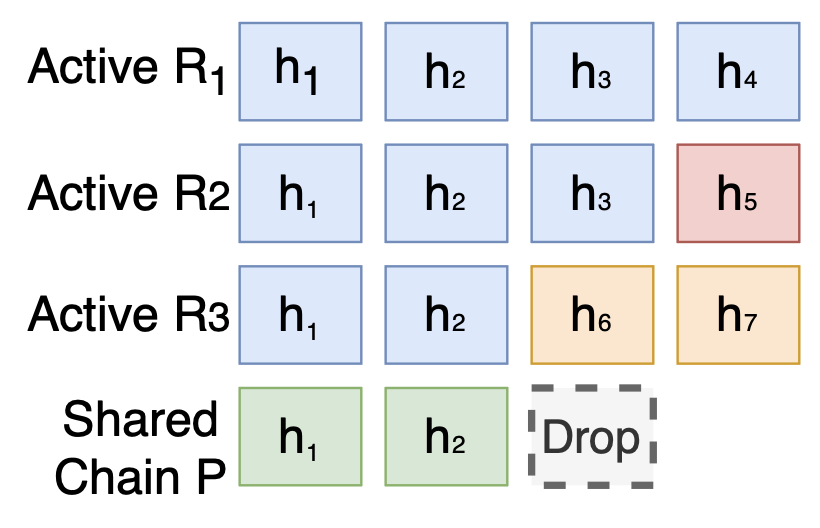
\includegraphics[width=\linewidth]{illustration_images/shared_prefix_chain_step3.png}
    \caption{}
    \label{fig:shared_prefix_chain_step3}
\end{subfigure}
\hfill
\begin{subfigure}{0.24\textwidth}
    \centering
    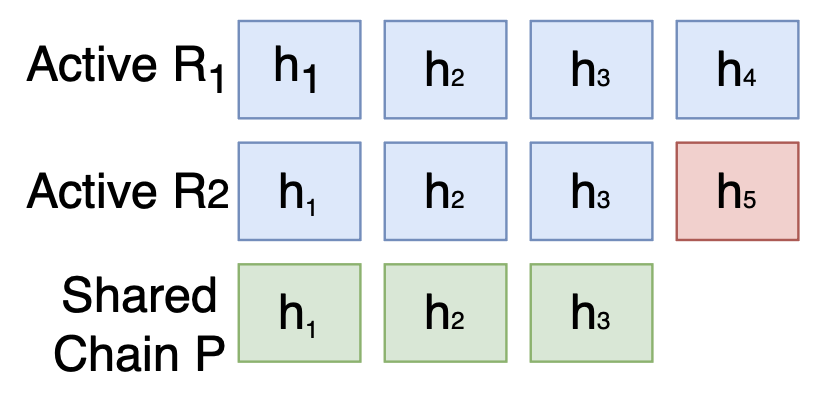
\includegraphics[width=\linewidth]{illustration_images/shared_prefix_chain_step4.png}
    \caption{}
    \label{fig:shared_prefix_chain_step4}
\end{subfigure}

\caption{An example of shared prefix chain workflow. We initially have just a single active request $R_1$ with four prefix hash chunks, so the shared prefix chain is also the same as its hash vector, as shown in figure~\ref{fig:shared_prefix_chain_step1}. We then activate $R_2$, which does not have the last level common with $R_1$, and thus the chain size reduces by one~\ref{fig:shared_prefix_chain_step2}. Similarly, as shown in~\ref{fig:shared_prefix_chain_step3}, activation of another request $R_3$ leads to further reduction in the chain size. Now, $R_3$ finishes its execution first, so we remove it from the set of active requests, and therefore this gives an opportunity to extend the chain~\ref{fig:shared_prefix_chain_step4}.}
\label{fig:shared_prefix_chain_workflow}
\end{figure*}


\subsubsection*{Optimizations}
\paragraph{Result caching.}
$\textsc{FindBest}()$ may be called repeatedly within a single scheduling round without any intervening state change.  We cache its last result—a four-tuple\\ $(r^*, \mathit{chunks\_before}, \mathit{chunks\_after}, \mathit{peers})$ and return it immediately on subsequent calls until a mutation invalidates the flag. 

\paragraph{Lazy heap updates.}
The waiting heap uses \emph{lazy deletion}: when a request's missing count changes, we push a new $(m_r, r)$ entry rather than updating the existing one in place. Stale entries (where the recorded $m$ differs from $\mathit{miss}[r]$) are silently skipped during $\textsc{FindBest}$. This avoids the $O(W)$ cost of a linear heap search and keeps activation and completion at $O(C \cdot W_h \cdot \log W)$ total, where $W_h$ is the average number of waiting requests per hash.

\paragraph{Incremental shared prefix chain maintenance.}
Recomputing the shared prefix chain from scratch after every activate or finish event would cost $O(A \cdot C)$, where $A$ is the active-set size. Instead, we exploit the fact that activation can only \emph{shrink} the chain and completion can only \emph{grow} it. On activation, we truncate $P$ at the first mismatch with the new request's hash vector in $O(L)$; on completion, we attempt a forward extension beyond the current chain length, stopping at the first disagreement, again in $O(L + C_{\max})$.

Additionally, all major hash tables and vectors pre-allocate capacity at construction time, eliminating rehash latency and reallocation during high-throughput operation.

\subsubsection*{Complexity Analysis}
Table~\ref{tab:complexity} summarizes the time complexity of each operation. $T$ is the average number of tokens per request, $C$ is the average number of chunks per request, $W$ is the number of waiting requests, and $W_h$ is the average number of waiting requests sharing a given hash (typically $W_h \ll W$).

\begin{table}[H]
\centering
\caption{Time complexity of CHT scheduler operations.}
\label{tab:complexity}
\begin{tabular}{ll}
\hline
\textbf{Operation} & \textbf{Complexity}\\
\hline
Insert request            & $O(T + C \log W)$ \\
Activate request          & $O(C \cdot W_h \cdot \log W)$ \\
Update chain on activate  & $O(L)$ \\
Finish request            & $O(C \cdot W_h \cdot \log W)$ \\
Update chain on finish    & $O(L + C_{\max})$ \\
Find best request         & $O(\log W)$ (cached: $O(1)$) \\
Remove request            & $O(C)$ \\
\hline
\end{tabular}
\end{table}

Here $L \le C$ is the current shared chain length, and $C_{\max}$ is the maximum number of chunks in any active request. Because result caching eliminates redundant heap traversals between working-set changes, the dominant cost in practice is the $O(C \cdot W_k \cdot \log W)$ propagation step in activate and finish, which updates the missing counts of all affected waiting requests.

\subsection{Batching and Reinforcement Learning}
\textcolor{red}{any visualizations for these RL policies needed?}

So far, the CHT provides us with an efficient way to find the best next request to add to the batch, the one that maximizes prefix reuse. But it does not tell us \emph{when to stop}. Adding more requests always increases GPU utilization, but at some point, the shared prefix starts to shrink, hurting locality. This section describes how we frame this stop/continue decision as a learning problem and present three policies of increasing complexity: a hand-crafted heuristic that encodes domain intuition, a contextual bandit that learns from experience without temporal structure, and a Q-learning agent that reasons about long-term throughput.

As highlighted in \S\ref{sec:system_overview}, the scheduler incrementally builds a decoding batch by repeatedly selecting the lowest-cost waiting request via the CHT and deciding whether to add it to the current batch or dispatch the batch as-is. This stop/continue decision is the crux of the batching problem. 

\subsubsection*{State, Actions, and Reward}
At each step of batch formation, the scheduler observes a state
\[
s = (\mathit{batch\_size},\; \mathit{chunks\_before},\; \mathit{chunks\_after},\;\mathit{requests\_waiting})
\]
and takes a binary action $a \in \{\textsc{Add}, \textsc{Stop}\}$. Here, $\mathit{batch\_size}$ denotes the number of requests that are already in the batch, which is a proxy for current GPU utilization. $\mathit{chunks\_before}$ is the shared-prefix chain length \emph{before} adding the candidate request; $\mathit{chunks\_after}$ is the chain length after hypothetically adding it (obtained from $\textsc{FindBest}$); and $\mathit{requests\_waiting}$ is the number of waiting requests that share the prefix up to level $\mathit{chunks\_after}$, indicating whether the locality cost of this addition will be compensated by future activations. Together, these four values capture both the current GPU utilization (batch size) and the cost of the proposed addition to prefix locality, summarized by the chunk loss $\Delta = \mathit{chunks\_before} - \mathit{chunks\_after}$).

Both learning policies share the same reward signal: the decode throughput of the dispatched batch,

\[
\mathcal{R} = \text{throughput}_{\mathrm{decode}}
\]

Maximizing this reward simultaneously encourages large batches (better GPU utilization) and short decode times (better prefix locality). Both policies also operate over the same discretized state space: $\mathit{batch\_size}$ and $\mathit{requests\_waiting}$ are mapped to exponential bins, while the chunk loss $\Delta$ is mapped to a coarser set of thresholds. The discretized state is a triple $(\hat{b}, \hat{\Delta}, \hat{w})$, where each hat denotes the bin index. The resulting table is small enough to store in a hash map and converges quickly, even under moderate traffic.

\subsubsection*{Heuristic Policy}
Before introducing any learning, we establish a baseline that encodes domain intuition directly as rules. The heuristic is designed around two competing goals: \emph{maximizing GPU utilization} by filling the batch as much as possible and \emph{preserving prefix locality} by avoiding candidates that cause large drops in the shared prefix chain. The heuristic always adds a candidate that does not hurt the shared chain at all—a free addition. When the batch is still very small and GPU utilization is clearly low, it tolerates a slightly larger locality cost to avoid dispatching an underutilized batch. In the general case, it accepts a candidate only if the chunk loss is within a small tolerance. Finally, when many waiting requests share the same prefix level, it allows a marginally higher locality cost since the short-term penalty is likely to be offset by the homogeneous additions that follow. If none of these conditions are met, the heuristic stops and dispatches the current batch.

This policy requires no training and converges immediately, but its thresholds are fixed and cannot adapt to shifts in workload distribution.

\subsubsection*{Contextual Bandit}
To move beyond hand-tuned thresholds, we implement a contextual bandit using Upper Confidence Bound (UCB) selection~\cite{auer2002finite}. The bandit treats each batch-construction call as an independent decision: given the discretized state $\hat{s} = (\hat{b}, \hat{\Delta}, \hat{w})$, it selects the action that maximizes
\[
  \mathrm{UCB}(\hat{s},a) = \frac{\mu(\hat{s},a)}{n(\hat{s},a)} + c\sqrt{\frac{\ln N}{n(\hat{s},a)}}
\]
where $\mu(\hat{s}, a)$ is the cumulative reward for taking action $a$ in state $\hat{s}$, $n(\hat{s}, a)$ is the number of times that pair has been selected, $N$ is the total number of steps, and $c$ is the exploration coefficient. The first term favors actions that have historically yielded high throughput; the second term ensures that under-explored actions are tried sufficiently often.

Because the bandit discards temporal structure entirely, it does not reason about how today's batching decision affects the state of the queue for the next batch, it can miss opportunities where a short-term locality sacrifice leads to a better-amortized sequence of future batches. This motivates the full reinforcement learning approach.

\subsubsection*{Q-Learning Policy}
To capture the temporal dependencies that the bandit ignores, we model batch construction as an episodic reinforcement learning problem. A new episode begins each time the scheduler starts forming a fresh batch and terminates when it issues \textsc{Stop} or the waiting queue is exhausted. The Q-table~\cite{watkins1992} stores a value $Q(s, a)$ for every (discretized state, action) pair and is updated upon each batch completion via the standard Bellman update:

\[
Q(s, a) \; \leftarrow\; Q(s, a) + \alpha\bigl[r + \gamma \max_{a'} Q(s', a') - Q(s, a)\bigr]
\]

where $r$ is the observed throughput reward, $s'$ is the state at the start of the \emph{next} batch formation, $\alpha$ is the learning rate, and $\gamma$ is the discount factor. The discount factor encodes that the agent values near-term throughput slightly more than long-term gains, which matches the real-time nature of an inference server. During training, $\varepsilon$ starts at $1.0$ (fully random) and decays linearly to $\varepsilon_{\min}$ over a configurable number of steps, after which the policy is nearly deterministic.

\subsubsection*{The \textsc{BuildBatch} Procedure}
Algorithm~\ref{alg:rl_batch} shows how all three policies fit into the same batch-construction loop. At each iteration, \textsc{FindBest} (Algorithm~\ref{alg:find_best}) is called to retrieve the lowest-cost candidate from the CHT along with its chain statistics $c_{\mathrm{before}}$, $c_{\mathrm{after}}$, and the number of waiting requests $w$ that share the same prefix level. These four values are assembled into the state $s$ and passed to whichever policy $\pi$ is active—heuristic, bandit, or Q-learning agent—which returns either \textsc{Add} or \textsc{Stop}. If \textsc{Add}, the candidate is activated and appended to the batch; if \textsc{Stop}, the loop exits and the batch is dispatched immediately. Once the batch executes, the observed decode throughput serves as the reward signal: the bandit updates its count-and-mean tables, while the Q-learning agent applies the Bellman update above. The heuristic requires no update. 

\begin{algorithm}[H]
\caption{$\textsc{BuildBatch}()$}
\label{alg:rl_batch}
\begin{algorithmic}[1]
\Require Waiting queue $Q$; policy $\pi$ (heuristic, bandit, or Q-learning); discount $\gamma$; learning rate $\alpha$
\Ensure Batch $B$ ready for one decode iteration
\State $B \gets \emptyset$
\While{$Q \neq \emptyset$}
    \State $(r^*, c_{\mathrm{before}}, c_{\mathrm{after}}, w) \gets \textsc{FindBest}()$
    \If{$r^* = \bot$} \textbf{break} \EndIf
    \State $s \gets (|B|,\; c_{\mathrm{before}},\; c_{\mathrm{after}},\; w)$
    \State $a \gets \pi(s)$ \Comment{heuristic rule / UCB look-up / $\varepsilon$-greedy Q-table}
    \If{$a = \textsc{Stop}$} \textbf{break} \EndIf
    \State $\textsc{Activate}(r^*)$;\quad $B \gets B \cup \{r^*\}$
\EndWhile
\State $\text{throughput}_{\mathrm{decode}} \gets \textsc{ExecuteBatch}(B)$
\State \textbf{Update} $\pi$ with observed reward $\text{throughput}_{\mathrm{decode}}$ \Comment{no-op for heuristic}
\State \Return $B$
\end{algorithmic}
\end{algorithm}






\subsection{Integration with vLLM and SGLang}
We integrate our scheduler as a lightweight layer on top of both vLLM's~\cite{kwon2023efficient} and SGLang's~\cite{zheng2024sglangefficientexecutionstructured} existing request management pipeline. The Chunked Hash Tree (implemented in C++), shared prefix chain tracking, and reinforcement learning policies operate entirely at the scheduler level.